
\definecolor{cb3b3b3}{RGB}{179,179,179}
\definecolor{c214478}{RGB}{33,68,120}


\begin{tikzpicture}[y=0.80pt, x=0.8pt,yscale=-1, inner sep=0pt, outer sep=0pt]
\begin{scope}[shift={(0,-782.35975)}]
  \begin{scope}[shift={(0,774.35975)},fill=black]
  \end{scope}
  \path[fill=cb3b3b3] (551.6854,1030.9418) -- (555.1986,1037.0269) --
    (551.7523,1042.9960) -- cycle;
  \path[draw=cb3b3b3,line join=miter,line cap=butt,miter limit=4.00,line
    width=1.600pt] (310.2661,803.7281) -- (310.2661,1036.9689)(552.6553,1036.9689)
    -- (310.2661,1036.9689);
  \path[fill=cb3b3b3] (304.2390,807.7175) -- (310.3241,804.2043) --
    (316.2932,807.6506) -- cycle;
  \path[color=black,fill=cb3b3b3,line width=0.800pt] (499.8557,820.2697) --
    (500.8557,820.2697) -- (500.8557,808.2697) -- (499.8557,808.2697) --
    cycle(499.8557,844.2697) -- (500.8557,844.2697) -- (500.8557,832.2697) --
    (499.8557,832.2697) -- cycle(499.8557,868.2697) -- (500.8557,868.2697) --
    (500.8557,856.2697) -- (499.8557,856.2697) -- cycle(499.8557,892.2697) --
    (500.8557,892.2697) -- (500.8557,880.2697) -- (499.8557,880.2697) --
    cycle(499.8557,916.2697) -- (500.8557,916.2697) -- (500.8557,904.2697) --
    (499.8557,904.2697) -- cycle(499.8557,940.2697) -- (500.8557,940.2697) --
    (500.8557,928.2697) -- (499.8557,928.2697) -- cycle(499.8557,964.2697) --
    (500.8557,964.2697) -- (500.8557,952.2697) -- (499.8557,952.2697) --
    cycle(499.8557,988.2697) -- (500.8557,988.2697) -- (500.8557,976.2697) --
    (499.8557,976.2697) -- cycle(499.8557,1012.2698) -- (500.8557,1012.2698) --
    (500.8557,1000.2697) -- (499.8557,1000.2697) -- cycle(499.8557,1036.2696) --
    (500.8557,1036.2696) -- (500.8557,1024.2696) -- (499.8557,1024.2696) -- cycle;
  \path[fill=cb3b3b3] (254.6422,1030.9418) -- (258.1554,1037.0269) --
    (254.7091,1042.9960) -- cycle;
  \path[draw=cb3b3b3,line join=miter,line cap=butt,miter limit=4.00,line
    width=1.600pt] (13.2229,803.7281) -- (13.2229,1036.9689)(255.6121,1036.9689)
    -- (13.2229,1036.9689);
  \path[fill=cb3b3b3] (7.1958,805.5497) -- (13.2809,802.0365) --
    (19.2500,805.4828) -- cycle;
  \path[color=black,fill=cb3b3b3,line width=0.800pt] (202.8125,820.2697) --
    (203.8125,820.2697) -- (203.8125,808.2697) -- (202.8125,808.2697) --
    cycle(202.8125,844.2697) -- (203.8125,844.2697) -- (203.8125,832.2697) --
    (202.8125,832.2697) -- cycle(202.8125,868.2697) -- (203.8125,868.2697) --
    (203.8125,856.2697) -- (202.8125,856.2697) -- cycle(202.8125,892.2697) --
    (203.8125,892.2697) -- (203.8125,880.2697) -- (202.8125,880.2697) --
    cycle(202.8125,916.2697) -- (203.8125,916.2697) -- (203.8125,904.2697) --
    (202.8125,904.2697) -- cycle(202.8125,940.2697) -- (203.8125,940.2697) --
    (203.8125,928.2697) -- (202.8125,928.2697) -- cycle(202.8125,964.2697) --
    (203.8125,964.2697) -- (203.8125,952.2697) -- (202.8125,952.2697) --
    cycle(202.8125,988.2697) -- (203.8125,988.2697) -- (203.8125,976.2697) --
    (202.8125,976.2697) -- cycle(202.8125,1012.2698) -- (203.8125,1012.2698) --
    (203.8125,1000.2697) -- (202.8125,1000.2697) -- cycle(202.8125,1036.2696) --
    (203.8125,1036.2696) -- (203.8125,1024.2696) -- (202.8125,1024.2696) -- cycle;
  \path[fill=black] (195.51093,1048.4893) node[above right] (text3075-4-1-2-9)
    {$0.0$};
  \path[fill=black] (260.02991,1040.9917) node[above right] (text3075-4-1-2-9-9)
    {$\frac{r}{R}$};
  \path[fill=black] (7.1002321,798.70367) node[above right] (text3075-4-1-2-9-9-7)
    {$v$};
  \path[fill=black] (300.88107,801.44177) node[above right]
    (text3075-4-1-2-9-9-7-1) {$\tau$};
  \path[fill=black] (487.5376,1048.4893) node[above right] (text3075-4-1-2-9-70)
    {$0.0$};
  \path[fill=black] (558.79633,1040.6738) node[above right] (text3075-4-1-2-9-9-5)
    {$\frac{r}{R}$};
  \path[fill=black] (1.7341394,1048.0874) node[above right] (text3075-4-1-2-9-91)
    {$1.0$};
  \path[fill=black] (293.76083,1048.0874) node[above right]
    (text3075-4-1-2-9-70-9) {$1.0$};
  \path[shift={(0,782.35975)},draw=c214478,line join=miter,line cap=butt,line
    width=0.800pt] (13.1755,254.6286) .. controls (60.3876,127.9977) and
    (91.1303,26.2538) .. (203.1219,26.2538);
  \path[shift={(0,782.35975)},draw=c214478,dash pattern=on 3.20pt off 1.60pt,line
    join=miter,line cap=butt,miter limit=4.00,line width=0.800pt]
    (13.1755,254.2626) .. controls (13.1755,25.8814) and (13.0521,25.8878) ..
    (203.4878,25.8878);
  \path[shift={(0,782.35975)},fill=black] (52.701889,186.92133) node[above right]
    (text3912)
    {$v=v_{max}\left[1-\left(\frac{r}{R}\right)^{2}\right]\;\;\&\;\;\frac{\left\langle
    v\right\rangle }{v_{max}}=\frac{1}{2}$};
  \path[fill=black] (28.805967,872.54803) node[above right] (text3916)
    {$v=v_{max}\left[1-\frac{r}{R}\right]^{\frac{1}{7}}\;\;\&\;\;\frac{\left\langle
    v\right\rangle }{v_{max}}=\frac{4}{5}$};
  \path[color=black,fill=cb3b3b3,line width=0.800pt] (435.3365,820.2697) --
    (436.3365,820.2697) -- (436.3365,808.2697) -- (435.3365,808.2697) --
    cycle(435.3365,844.2697) -- (436.3365,844.2697) -- (436.3365,832.2697) --
    (435.3365,832.2697) -- cycle(435.3365,868.2697) -- (436.3365,868.2697) --
    (436.3365,856.2697) -- (435.3365,856.2697) -- cycle(435.3365,892.2697) --
    (436.3365,892.2697) -- (436.3365,880.2697) -- (435.3365,880.2697) --
    cycle(435.3365,916.2697) -- (436.3365,916.2697) -- (436.3365,904.2697) --
    (435.3365,904.2697) -- cycle(435.3365,940.2697) -- (436.3365,940.2697) --
    (436.3365,928.2697) -- (435.3365,928.2697) -- cycle(435.3365,964.2697) --
    (436.3365,964.2697) -- (436.3365,952.2697) -- (435.3365,952.2697) --
    cycle(435.3365,988.2697) -- (436.3365,988.2697) -- (436.3365,976.2697) --
    (435.3365,976.2697) -- cycle(435.3365,1012.2698) -- (436.3365,1012.2698) --
    (436.3365,1000.2697) -- (435.3365,1000.2697) -- cycle(435.3365,1036.2696) --
    (436.3365,1036.2696) -- (436.3365,1024.2696) -- (435.3365,1024.2696) -- cycle;
  \path[color=black,fill=cb3b3b3,line width=0.800pt] (368.8137,818.7786) --
    (369.8137,818.7786) -- (369.8137,806.7786) -- (368.8137,806.7786) --
    cycle(368.8137,842.7786) -- (369.8137,842.7786) -- (369.8137,830.7786) --
    (368.8137,830.7786) -- cycle(368.8137,866.7786) -- (369.8137,866.7786) --
    (369.8137,854.7786) -- (368.8137,854.7786) -- cycle(368.8137,890.7786) --
    (369.8137,890.7786) -- (369.8137,878.7786) -- (368.8137,878.7786) --
    cycle(368.8137,914.7786) -- (369.8137,914.7786) -- (369.8137,902.7786) --
    (368.8137,902.7786) -- cycle(368.8137,938.7786) -- (369.8137,938.7786) --
    (369.8137,926.7786) -- (368.8137,926.7786) -- cycle(368.8137,962.7786) --
    (369.8137,962.7786) -- (369.8137,950.7786) -- (368.8137,950.7786) --
    cycle(368.8137,986.7786) -- (369.8137,986.7786) -- (369.8137,974.7786) --
    (368.8137,974.7786) -- cycle(368.8137,1010.7787) -- (369.8137,1010.7787) --
    (369.8137,998.7786) -- (368.8137,998.7786) -- cycle(368.8137,1034.7784) --
    (369.8137,1034.7784) -- (369.8137,1022.7785) -- (368.8137,1022.7785) -- cycle;
  \path[fill=black] (391.24301,905.7287) node[above right] (text4282)
    {$\substack{\text{buffer}\\ \tau^{\mu}\approx\tau^{t}}$};
  \path[fill=black] (324.52493,1006.7668) node[above right] (text4282-9)
    {$\substack{\text{laminar}\\ \text{sublayer}\\ \tau^{\mu}\gg\tau^{t}}$};
  \path[fill=black] (448.60583,852.25946) node[above right] (text4282-9-0)
    {$\substack{\text{turbulent}\\ \text{core}\\ \tau^{\mu}\ll\tau^{t}}$};
  \path[draw=c214478,line join=miter,line cap=butt,line width=0.800pt]
    (310.1642,1036.4540) .. controls (320.9337,886.3436) and (441.6611,808.3060)
    .. (500.5361,808.3060);
\end{scope}

\end{tikzpicture}
